\documentclass[a4paper,12pt]{article}
\usepackage{epsfig}
\usepackage{amssymb}
\usepackage{amsmath}
\usepackage{theorem}
\usepackage{rotating}
\usepackage[dvips]{color}
\usepackage[round]{natbib}
\usepackage{times}
\usepackage{color}
\usepackage{bbm}
\usepackage{fancyhdr}
\usepackage{ulem}
\usepackage{framed}
\usepackage{subfigure}

\setlength{\topmargin} {-1cm} %-1.5cm
\oddsidemargin  0.cm
\evensidemargin 0.cm
\setlength{\textwidth} {15.5cm}
\textheight 21.75cm
\setlength{\headsep} {1.5cm}

\parindent0mm


\newcommand{\mb}[1]{{\mbox{\boldmath$#1$\unboldmath}}}
\newcommand{\intd}{\,{\rm d}}
\newcommand{\p}{\partial}

\newcommand{\divergenz}{{\rm div}}
\newcommand{\Divergenz}{{\rm Div}}
\newcommand{\gradient}{{\rm grad}}
\newcommand{\Gradient}{{\rm Grad}}
\newcommand{\trace}{{\rm tr}}
\newcommand{\mydet}{\text{det}\,}
\newcommand{\myspat}{\text{spat}\,}
\newcommand{\sint}{\text{sin}\,}
\newcommand{\cost}{\text{cos}\,}

\newcounter{bild}
\newcommand{\Abb}[1]{\refstepcounter{bild}
                    {\footnotesize Figure \arabic{bild}: #1}}
\newcounter{tabelle}
\newcommand{\Tab}[1]{\refstepcounter{tabelle}
                    {\footnotesize Table \arabic{tabelle}: #1}}


% Hier ist der Kopf definiert. 
\pagestyle{fancy}

\headheight 40pt 
\lhead{
\begin{minipage}[c]{4cm}
Meriem Ben Salah\\
\end{minipage}
}
\rhead{
\begin{minipage}[c]{3.4cm}
Cut Cell 1D\\
\today\\
\end{minipage}
}


%\lfoot{Meriem }
\cfoot{\arabic{page}}


\begin{document}


\pagebreak

%\frontmatter
\setcounter{tabelle}{0}

\sloppy
\newpage
\setcounter{bild}{0} 
\section{Problem 1}
\subsection{Description}
We want to solve the following BVP:
\begin{eqnarray*}
Au_{,xx} &=& K,\\
A &=& 3,\\
K &=& 10,\\
u_{x=0} &=& 0,\\
0 &<& x < L,\\
L &=& 1.
\end{eqnarray*}
\subsection{Results}
\begin{center}
\scalebox{0.7}{\includegraphics{n4.eps}}\\
\scalebox{0.7}{\includegraphics{n8.eps}}\\
\scalebox{0.7}{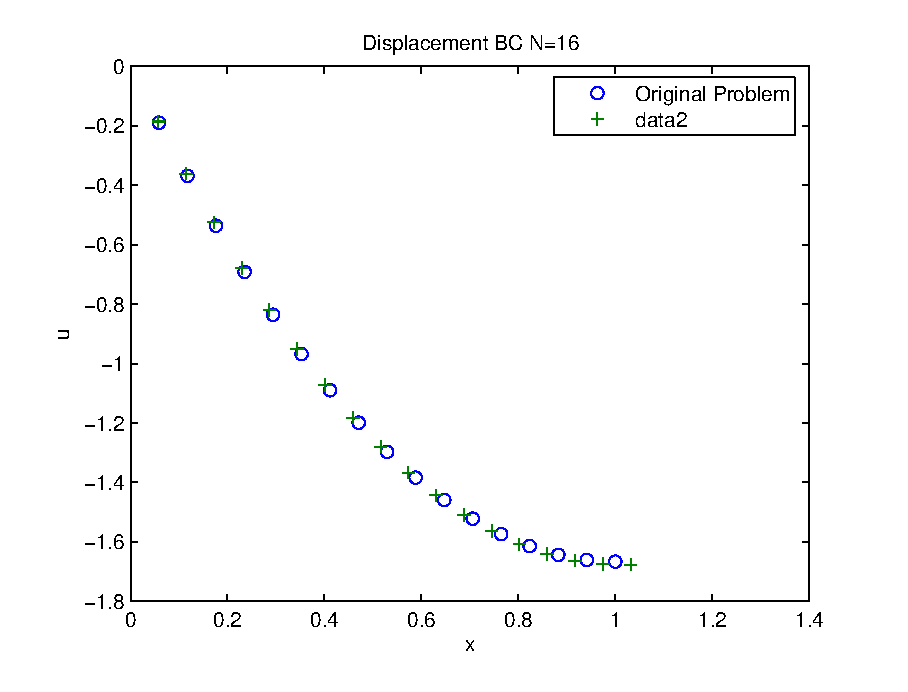
\includegraphics{n16.eps}}\\
\scalebox{0.7}{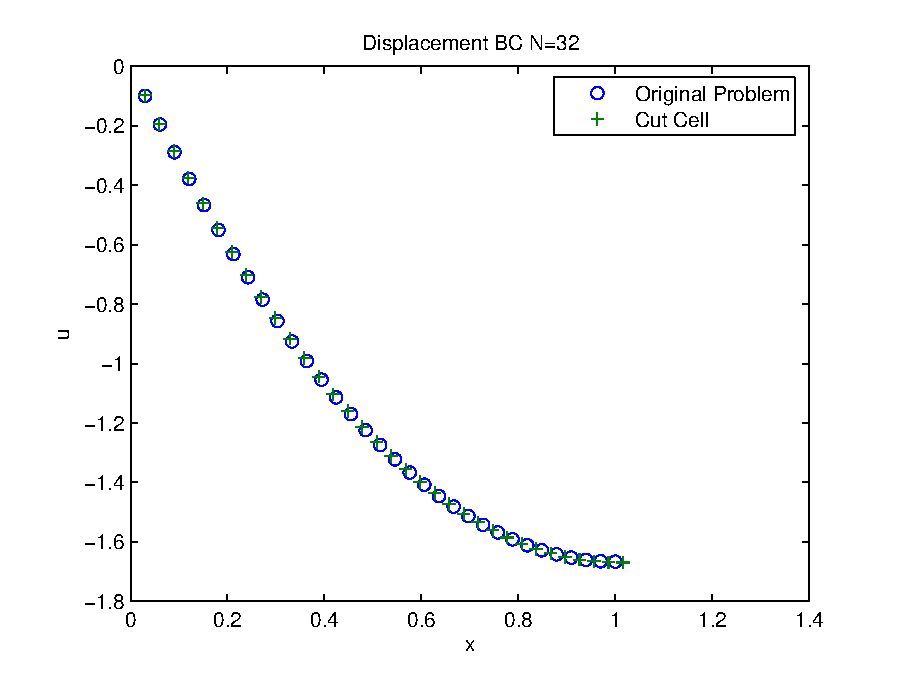
\includegraphics{n32.eps}}\\
\scalebox{0.7}{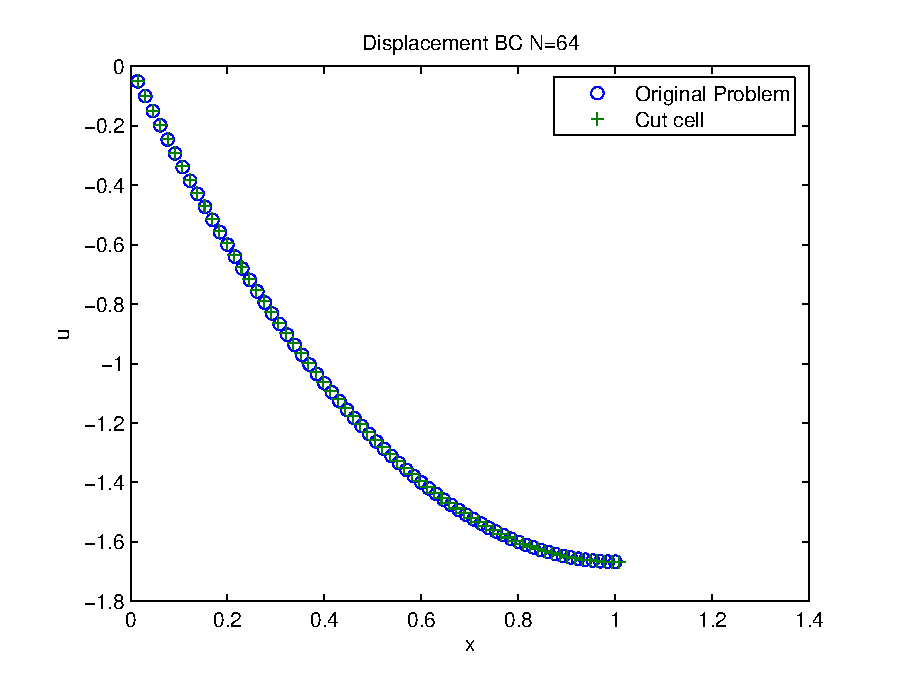
\includegraphics{n64.eps}}\\
\Abb{Convergence study for regular FEM vs. Cut Cell\footnote{The numerical integration of the last element is reduced to one gauss point.}}
\end{center}
\section{Problem 2}
\subsection{Description}
We want to solve the following BVP:
\begin{eqnarray*}
Au_{,xx} &=& 0,\\
A &=& 3,\\
u_{x=0} &=& 0,\\
0 &<& x < L,\\
L &=& 1,\\
Au_{,x}\vert_{x=L} &=& N,\\
N &=& -10.
\end{eqnarray*}
\subsection{Results}
\begin{center}
\scalebox{0.7}{\includegraphics{n4t.eps}}\\
\scalebox{0.7}{\includegraphics{n8t.eps}}\\
\scalebox{0.7}{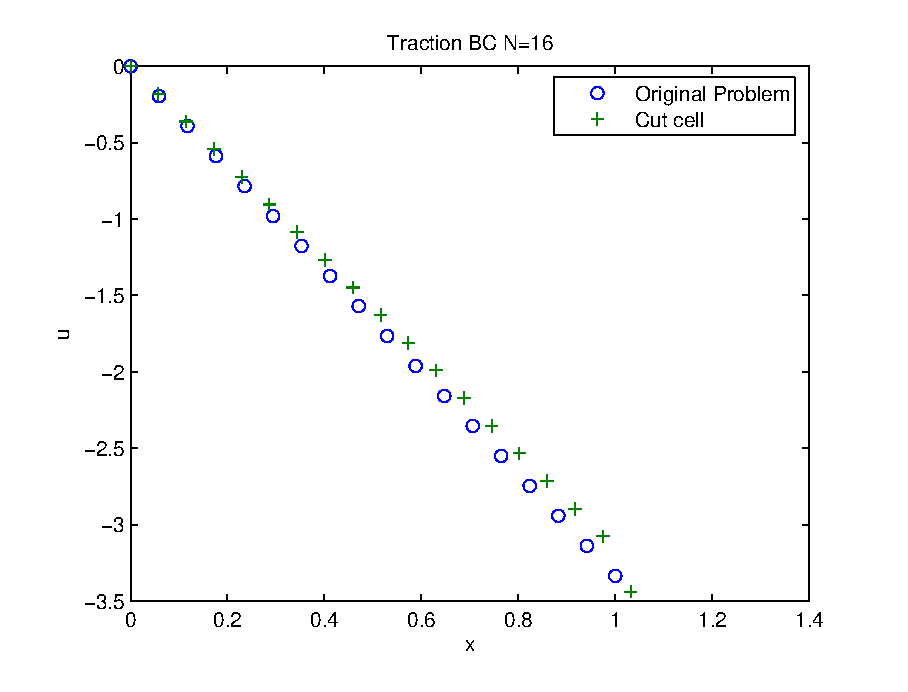
\includegraphics{n16t.eps}}\\
\scalebox{0.7}{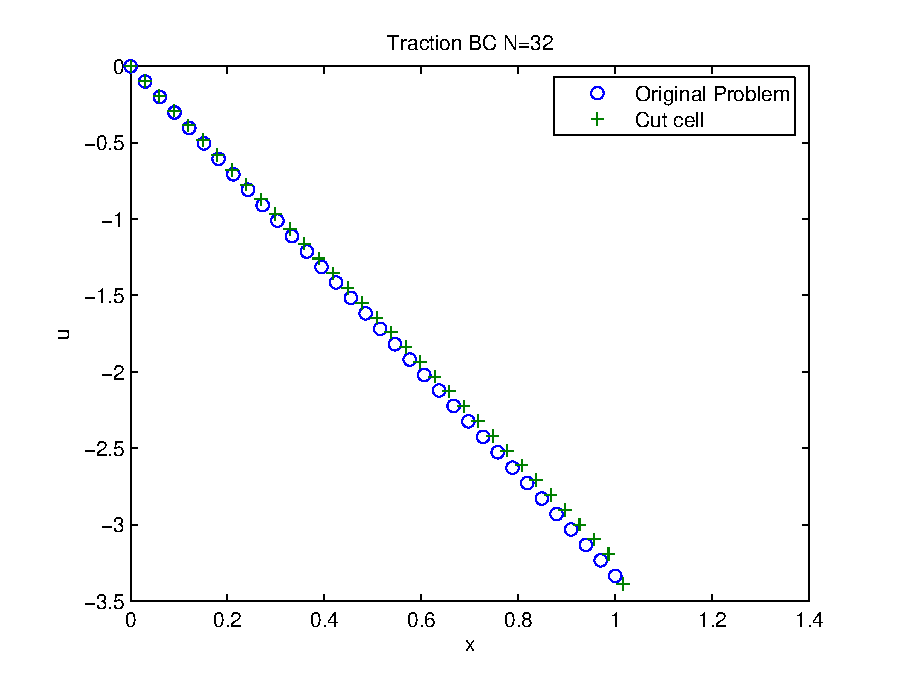
\includegraphics{n32t.eps}}\\
\scalebox{0.7}{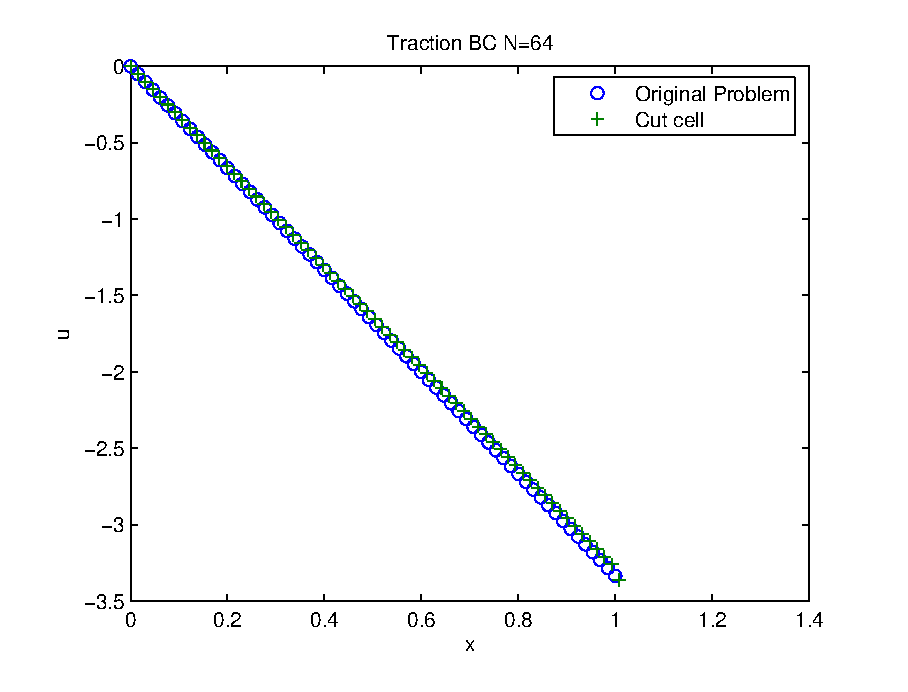
\includegraphics{n64t.eps}}\\
\scalebox{0.7}{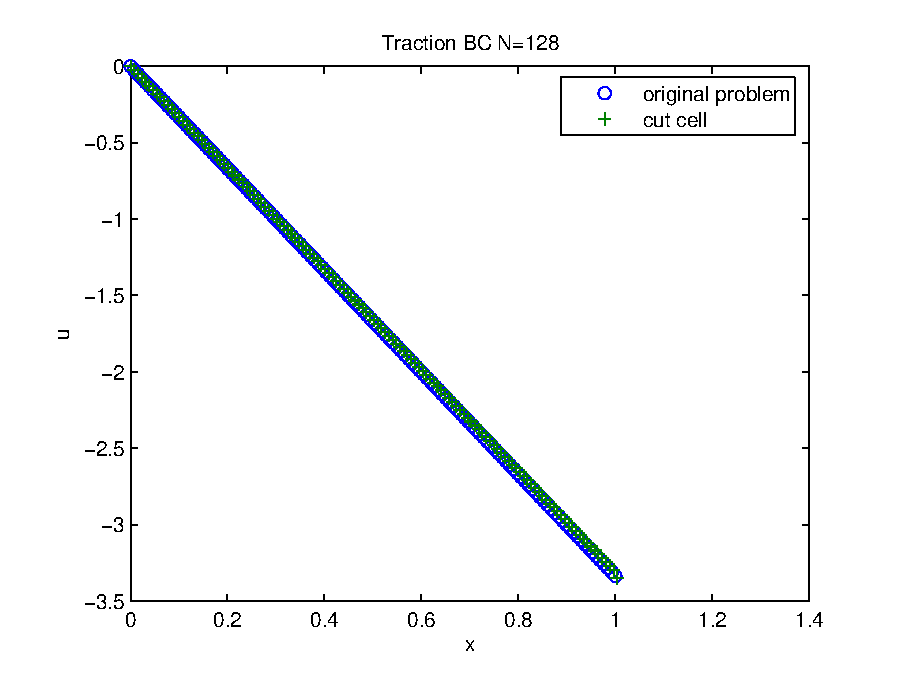
\includegraphics{n128t.eps}}\\
\Abb{Convergence study for regular FEM vs. Cut Cell}
\end{center}

\end{document}
%\begin{framed}
%\end{framed}
